
\documentclass{beamer}
\usecolortheme{dove}
\setbeamertemplate{navigation symbols}{}
\usepackage{amsmath,amssymb,amsfonts,amsthm, multicol, subfigure, color}
\usepackage{bm}
\usepackage{graphicx}
\usepackage{tabularx}
\usepackage{booktabs}
\usepackage{hyperref}
\usepackage{pdfpages}
\usepackage{xcolor}
\definecolor{seagreen}{RGB}{46, 139, 87}
\definecolor{seagreen4}{RGB}{46, 139, 87}
\def\independenT#1#2{\mathrel{\rlap{$#1#2$}\mkern2mu{#1#2}}}
\newcommand\indep{\protect\mathpalette{\protect\independenT}{\perp}}
\def\log{\text{log}}
\newcommand\logit{\text{logit}}
\newcommand\iid{\stackrel{\text{iid}}{\sim}}
\newcommand\E{\text{E}}
\newcommand\V{\text{V}}
\renewcommand\P{\text{P}}
\newcommand{\Cov}{\text{Cov}}
\newcommand{\Cor}{\text{Cor}}
\newcommand\doop{\texttt{do}}
\usepackage{stackrel}
\usepackage{tikz}
\usetikzlibrary{arrows,shapes.arrows,positioning,shapes,patterns,calc}
\newcommand\slideref[1]{\vskip .1cm \tiny \textcolor{gray}{{#1}}}
\newcommand\red[1]{\color{red}#1}
\newcommand\blue[1]{\color{blue}#1}
\newcommand\gray[1]{\color{gray}#1}
\newcommand\seagreen[1]{\color{seagreen}#1}
\newcommand\purple[1]{\color{purple}#1}
\newcommand\orange[1]{\color{orange}#1}
\newcommand\black[1]{\color{black}#1}
\newcommand\white[1]{\color{white}#1}
\newcommand\teal[1]{\color{teal}#1}
\newcommand\magenta[1]{\color{magenta}#1}
\newcommand\Fuchsia[1]{\color{Fuchsia}#1}
\newcommand\BlueGreen[1]{\color{BlueGreen}#1}
\newcommand\bblue[1]{\textcolor{blue}{\textbf{#1}}}
\newcommand\bred[1]{\textcolor{red}{\textbf{#1}}}
\newcommand\bgray[1]{\textcolor{gray}{\textbf{#1}}}
\newcommand\bgreen[1]{\textcolor{seagreen}{\textbf{#1}}}
\newcommand\bref[2]{\href{#1}{\color{blue}{#2}}}
\colorlet{lightgray}{gray!40}
\pgfdeclarelayer{bg}    % declare background layer for tikz
\pgfsetlayers{bg,main} % order layers for tikz
\newcommand\mycite[1]{\begin{scriptsize}\textcolor{darkgray}{(#1)}\end{scriptsize}}
\newcommand{\tcframe}{\frame{
%\small{
\only<1|handout:0>{\tableofcontents}
\only<2|handout:1>{\tableofcontents[currentsection]}}
%}
}
\usepackage{verbatim}

\usepackage[round]{natbib}
\bibliographystyle{humannat-mod}
\setbeamertemplate{enumerate items}[default]
\usepackage{mathtools}

\newcommand{\goalsframe}{\begin{frame}{Learning goals for today}
At the end of class, you will be able to:
\begin{enumerate}
\item Define positivity
\item Understand how positivity relates to the adjustment set
\item Make estimates for the feasible subpopulation
\item Begin translating ideas to actual data
\end{enumerate} \vskip .2in
\end{frame}}

\title{7. Positivity: The problem of empty cells}
\author{Ian Lundberg\\Cornell Info 6751: Causal Inference in Observational Settings\\Fall 2022}
\date{13 Sep 2022}

\begin{document}

\maketitle

\goalsframe

% BEGIN HOUSING ASSISTANCE PAPER SLIDES
\begin{frame}{Running example for today's discussion}
\centering
\includegraphics[width = .8\textwidth, trim = 0 7.6in 0 1in, clip]{figures/assistance_p1} \vskip .5cm
\begin{footnotesize}Journal of Policy Analysis and Management\\2021\end{footnotesize}
\end{frame}

\begin{frame}{Running example for today's discussion}

Does public housing protect families from eviction?

\end{frame}

\begin{frame}{Running example for today's discussion}
\begin{tikzpicture}[x = \textwidth, y = .9\textheight]
\node at (0,0)  {};
\node at (1,1) {};
% BEGIN TIMELINE AT BOTTOM
\node[anchor = south] at (.5,0) {
\begin{tikzpicture}[x = \textwidth / 17, y = .5\textheight, every node/.style={anchor = center}]
\draw[thick] (-1,.1) -- (16,.1);
\foreach \i in {0, 1,3,5,9,15} {
\draw[thick] (\i,.09) -- (\i,.11);
\node[font = \footnotesize, anchor = north] at (\i,.09) {\i};
}
\node[font = \footnotesize] at (7.5,0) {Child Age};
% Note the age 9-15 report
\draw[thick] (9,.2) -- (15,.2);
\node[anchor = north, font = \scriptsize, gray] (t_label) at (9,.38) {Treatment};
\draw[->, thick, gray] (t_label) -- (9,.22); 
\draw[thick, gray] (0,.28) -- (8.8,.27);
\node[font = \scriptsize, gray, fill = white] at (4.5,.27) {Covariates};
\node[font = \scriptsize, gray, fill = white] at (12,.27) {Outcome};
\node[font = \footnotesize] at (15,.2) {$\bullet$};
\node[anchor = north, font = \footnotesize] at (12,.2) {Were you evicted?};
%\node[font = \footnotesize, align  = center] (difficult) at (12,.4) {Very difficult\\to predict\\for individuals};
%\draw[->, thick] (difficult) -- (12,.25);
% Note the earlier reports
\foreach \i in {1,3,5,9} {
\draw[thick] (\i - 1,.2) -- (\i,.2);
\node[font = \footnotesize] at (\i,.2) {$\bullet$};
}
\end{tikzpicture}};
% END TIMELINE
%\node[anchor = north west] at (0,1) {Prediction for causal claims};
%\node[anchor = north west, font = \small] at (0,.95) {Outcome variable $Y$: Eviction};
%\node[anchor = north west, font = \large] at (0,.95) {Estimation via outcome modeling};
% Factual science table is its own tikzppicture
\node[anchor = north west] (factual) at (0,.9) {
\scalebox{.7}{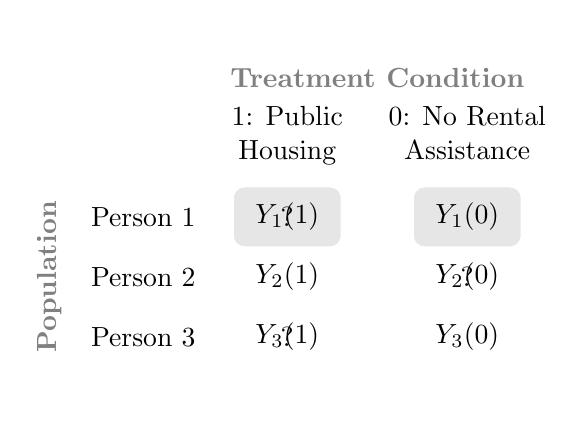
\begin{tikzpicture}[x = .9in, y = .3in, every node/.style={anchor = center}]
\node at (0,-4) {};
\node at (0,2) {};
\node[anchor = south, align = center, font = \bf, gray, rotate = 90] at (-.2,-2) {Population};
\node at (.2,-1) {Person 1};
\node at (.2,-2) {Person 2};
\node at (.2,-3) {Person 3};
\node[anchor = south, align = center, font = \bf, gray] at (1.5,1) {Treatment Condition};
\node[anchor = north, align = center] at (1,1) {1: Public\\Housing};
\node[anchor = north, align = center] at (2,1) {0: No Rental\\Assistance};
\draw<3,5>[color = white, fill = gray, fill opacity = .2, rounded corners] (.7,-1.5) rectangle (1.3,-.5);
\draw<4-5>[color = white, fill = gray, fill opacity = .2, rounded corners] (1.7,-1.5) rectangle (2.3,-.5);
\node<2-5> at (1,-1) {$Y_1(1)$};
\node<2-> at (2,-1) {$Y_1(0)$};
\node<2-> at (1,-2) {$Y_2(1)$};
\node<2-5> at (2,-2) {$Y_2(0)$};
\node<2-5> at (1,-3) {$Y_3(1)$};
\node<2-> at (2,-3) {$Y_3(0)$};
\node<6-> at (1,-1) {?};
\node<6-> at (2,-2) {?};
\node<6-> at (1,-3) {?};
\end{tikzpicture}}
};
% End factual science table
\node<7->[anchor = south, font = \small] (factual_label) at (factual.north) {Learn a prediction function};
\draw<7->[gray, line width = 1.2pt, line cap = round] (factual_label.south west) -- (factual_label.south east);
% Predicted science table is its own tikzppicture
\node<8->[anchor = north east] (predicted) at (1,.9) {
\scalebox{.7}{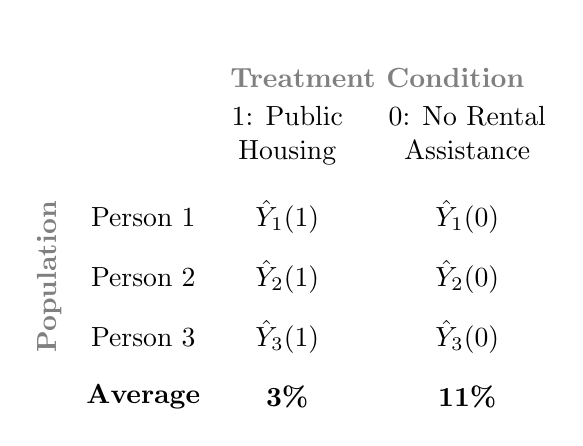
\begin{tikzpicture}[x = .9in, y = .3in, every node/.style={anchor = center}]
\node at (0,-4) {};
\node at (0,2) {};
\node[anchor = south, align = center, font = \bf, gray, rotate = 90] at (-.2,-2) {Population};
\node at (.2,-1) {Person 1};
\node at (.2,-2) {Person 2};
\node at (.2,-3) {Person 3};
\node[anchor = south, align = center, font = \bf, gray] at (1.5,1) {Treatment Condition};
\node[anchor = north, align = center] at (1,1) {1: Public\\Housing};
\node[anchor = north, align = center] at (2,1) {0: No Rental\\Assistance};
\node at (1,-1) {$\hat{Y}_1(1)$};
\node at (2,-1) {$\hat{Y}_1(0)$};
\node at (1,-2) {$\hat{Y}_2(1)$};
\node at (2,-2) {$\hat{Y}_2(0)$};
\node at (1,-3) {$\hat{Y}_3(1)$};
\node at (2,-3) {$\hat{Y}_3(0)$};
%\draw[thick] (.65,-.5) -- (.65,-3.5);
%\draw[thick] (.65,-.5) -- (2.4,-.5);
% Averages that appear on last slides
%\draw<13->[thick] (-.1,-3.5) -- (2.4,-3.5);
\node<13->[font = \bf] at (.2,-4) {Average};
%\draw<13>[thick] (.65,-3.5) -- (.65,-4.5);
\node<13->[font = \bf] at (1,-4) {3\%};
\node<14->[font = \bf] at (2,-4) {11\%};
\end{tikzpicture}}
};
% End predicted science table
\node<8->[anchor = south, font = \small] (predicted_label) at (predicted.north) {Predict the whole table};
\draw<8->[gray, line width = 1.2pt, line cap = round] (predicted_label.south west) -- (predicted_label.south east);
\node<8>[gray, font = \footnotesize, align  = right, anchor = south east] at (1,.4) {Robins 1986\\Hahn 1998};
% Begin DAG
\node<9->[font = \scriptsize, align = center] (x) at (.1,.37) {Measured\\Confounders};
\node<9->[font = \footnotesize, align = center] (t) at (.3,.37) {Public\\Housing};
\node<9->[font = \scriptsize] (y) at (.5,.37) {Eviction};
\draw<9->[->, thick] (x) -- (t);
\draw<9->[->, thick] (x) to[bend right] (y);
\draw<9->[->, thick] (t) -- (y);
\node<10>[font = \scriptsize, red] (u) at (.4,.47) {$U$};
\draw<10>[->, thick, dashed, red] (u) -- (t);
\draw<10>[->, thick, dashed, red] (u) -- (y);
%\node<11>[font = \footnotesize, seagreen4] (u) at (.3,.35) {$U$};
%\draw<11>[->, thick, dashed, seagreen4] (u) -- (x);
%\draw<11>[->, thick, dashed, seagreen4] (u) -- (y);
\node<11>[font = \scriptsize, seagreen4] (u1) at (.3,.47) {$U_1$};
\draw<11>[->, thick, dashed, seagreen4] (u1) -- (t);
\node<11>[font = \scriptsize, seagreen4] (u2) at (.5,.47) {$U_2$};
\draw<11>[->, thick, dashed, seagreen4] (u2) -- (y);
\node<12->[font = \scriptsize, align = center, gray] (this_pop) at (.5,.5) {Those\\factually in\\public housing};
\draw<12->[->, thick, gray] (this_pop) to[bend left] (.55,.6);
\end{tikzpicture}
\end{frame}

%\goalsframe

\begin{frame}{Setting 1: A highly simplified DAG} \pause

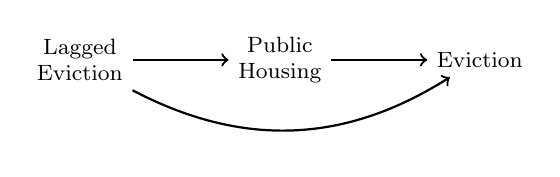
\begin{tikzpicture}[x = 1in, y = .5in]
\node[align = center, font = \footnotesize] (lag) at (-1,0) {Lagged\\Eviction};
\node[align = center, font = \footnotesize] (a) at (0,0) {Public\\Housing};
\node[align = center, font = \footnotesize] (y) at (1,0) {Eviction};
\draw[->, thick] (lag) -- (a);
\draw[->, thick] (a) -- (y);
\draw[->, thick] (lag) to[bend right] (y);
\end{tikzpicture} \pause

\bgray{Question:} How would you estimate in this setting?\vskip .1in
--- Caveat: Your method must be nonparametric (no regression) \pause \vskip .3in
\begin{enumerate}\small
\item Among those with (lagged eviction = TRUE), estimate the effect
\item Among those with (lagged eviction = FALSE), estimate the effect
\item Take a weighted average of the two estimates, weighted by the number of cases in each group
\end{enumerate}

\end{frame}

\begin{frame}[fragile]{Nonparametric estimation: In R code}
\footnotesize \pause
\begin{verbatim}
# Load packages
library(tidyverse)

# Simulate some data
sim_data <- data.frame(x1 = rbinom(n,1,.5),
                       x2 = rbinom(n,1,.5),
                       x3 = rbinom(n,1,.5)) %>%
  # Generate the treatment
  mutate(a = rbinom(n,1,plogis(x1 + x2 + x3))) %>%
  # Generate the outcome
  mutate(y = rnorm(n, x1 + x2 + x3 + a))
\end{verbatim}
\end{frame}

\begin{frame}[fragile]{Nonparametric estimation: In R code}
\footnotesize
\begin{verbatim}
# Define the confounders
confounders <- c("x1","x2","x3")

# Count cases in each stratum
strata_counts <- sim_data %>%
  # Group by the confounders
  group_by(across(all_of(confounders))) %>%
  # Count the number of cases
  summarize(cases = n(),
            .groups = "drop")
\end{verbatim}
\end{frame}

\begin{frame}[fragile]{Nonparametric estimation: In R code}
\footnotesize
\begin{verbatim}
# Estimate effect in each stratum
strata_effects <- sim_data %>%
  # Group by the confounders and treatment
  group_by(a, across(all_of(confounders))) %>%
  # Estimate the mean outcome
  summarize(ybar = mean(y),
            .groups = "drop") %>%
  # Prepare to make the data wider by re-valuing the treatment
  mutate(a = paste0("ybar_",a)) %>%
  # Make the data wide
  pivot_wider(names_from = "a", values_from = "ybar") %>%
  # Estimate the effect
  mutate(conditional_effect = ybar_1 - ybar_0)
\end{verbatim}
The \texttt{pivot\_wider} step makes a conversion like this:
\begin{tabular}{lll}
Stratum & a & ybar \\
\hline
1 & ybar\_1 & 3.6 \\
1 & ybar\_0 & 3.2 \\
2 & ybar\_1 & 3 \\
2 & ybar\_0 & 2.8 \\
$\vdots$ & $\vdots$ & $\vdots$
\end{tabular}\quad $\rightarrow$ \quad \begin{tabular}{llll}
Stratum & ybar\_1 & ybar\_0 \\
\hline
1 & 3.6 & 3.2 \\
2 & 3 & 2.8\\
$\vdots$ & $\vdots$ & $\vdots$
\end{tabular}
\end{frame}

\begin{frame}[fragile]{Nonparametric estimation: In R code}
\footnotesize
\begin{verbatim}
# Aggregate over strata
strata_counts %>%
  # Merge the effects into the counts data frame
  full_join(strata_effects, by = confounders) %>%
  # Stop working within strata. Average the effect
  ungroup() %>%
  summarize(average_effect = weighted.mean(conditional_effect, 
                                           w = cases))
\end{verbatim}
\end{frame}

\begin{frame}{Setting 2: A slightly more complex DAG}

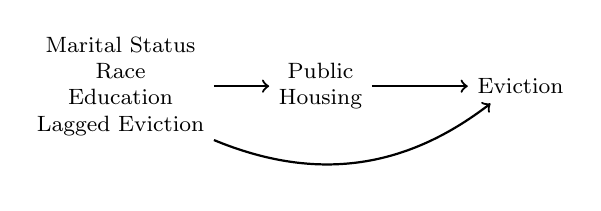
\begin{tikzpicture}[x = 1in, y = .5in]
\node[align = center, font = \footnotesize] (lag) at (-1,0) {Marital Status\\Race\\Education\\Lagged Eviction};
\node[align = center, font = \footnotesize] (a) at (0,0) {Public\\Housing};
\node[align = center, font = \footnotesize] (y) at (1,0) {Eviction};
\draw[->, thick] (lag) -- (a);
\draw[->, thick] (a) -- (y);
\draw[->, thick] (lag) to[bend right] (y);
\end{tikzpicture}

\bgray{Question:} How would you estimate in this setting?\vskip .1in
--- Caveat: Your method must be nonparametric (no regression) \pause \vskip .2in
\begin{enumerate}\small
\item In each subgroup defined by the covariates, estimate the effect
\item Take a weighted average of the two estimates, weighted by the number of cases in each group
\end{enumerate} \pause \vskip .1in
\bred{PROBLEM:} In some subgroups, the treatment does not vary

\end{frame}

\begin{frame}{To discuss}
\bgray{Situation:} In some subgroups, the treatment does not vary \vskip .2in
\bgray{Example:} (oversimplified for concreteness) \vskip .1in
When a mother has a college degree,\\
her family is never seen in public housing
 \vskip .2in
\bgray{Discuss:} Does causal inference make sense for this subgroup
\begin{enumerate}
\item if this happens in the sample but not the population?
\item if this happens in the sample and in the population?
\end{enumerate}
If it makes sense, how might you go about it?

\end{frame}

\begin{frame}{Positivity assumption (in the population)}

$$\P(A = a\mid \vec{L} = \vec\ell) > 0$$
for all treatment values $a$ in the causal estimand\\
and\\
for every covariate stratum $\vec\ell$ in the population of interest \pause \vskip .4in
Guarantees that in an infinite sample you will eventually see the needed treatment values

\end{frame}

\begin{frame}{Positivity assumption (in the population)}

A few examples where positivity would not hold: \pause
\begin{itemize}
\item Among 65-year-old teachers, how much would the earnings go up if they became a pitcher in Major League Baseball?
\begin{itemize} \pause
\item Nonsensical: No 65-year-old can be a pitcher
\end{itemize} \pause
\item Among bulbs planted in Ithaca, would the spring blooms change if it never froze all winter?
\begin{itemize} \pause
\item Nonsensical: It always freezes in Ithaca
\end{itemize} \pause
\item Among employees at Microsoft, what is the effect on productivity of searching using Bing vs.~Google?
\begin{itemize} \pause
\item Nonsensical: At Microsoft, they all use Bing
\end{itemize}
\end{itemize} \pause
You can theorize about these questions.\pause \\
But they will never happen---in an infinite sample, you'd never learn the answer.

\end{frame}

\begin{frame}{Empirical positivity (in the sample)} \pause

An empirical version of positivity:
\begin{itemize}
\item Within our sample, we observe every treatment value $a$ within every covariate stratum $\vec\ell$
\end{itemize} \pause \vskip .2in
Note:
\begin{itemize}
\item Empirical positivity implies theoretical positivity
\begin{itemize}
\item If we saw all treatments in this subgroup in our sample, they must exist in the population
\end{itemize} \pause
\item A lack of empirical positivity does not imply a lack of theoretical positivity
\begin{itemize}
\item All the treatment values may exist in this subgroup, and our sample just happened to miss them
\end{itemize}
\end{itemize}

\end{frame}

\begin{frame}{Feasible subsample (and subpopulation)}

(No empirical positivity) $\rightarrow$ (No nonparametric SATE estimator) \vskip .1in
where SATE is the Sample Average Treatment Effect. \pause \vskip .4in
But we can get FSATE: Feasible Sample Average Treatment Effect \vskip .1in
\begin{itemize}
\item The effect averaged over strata where all treatment values are observed
\end{itemize} \pause
We will go do this in R.

\end{frame}

\begin{frame}{Lots of confounders: Empirical positivity dies} \pause

Suppose we have the full adjustment set: \vskip .1in \pause
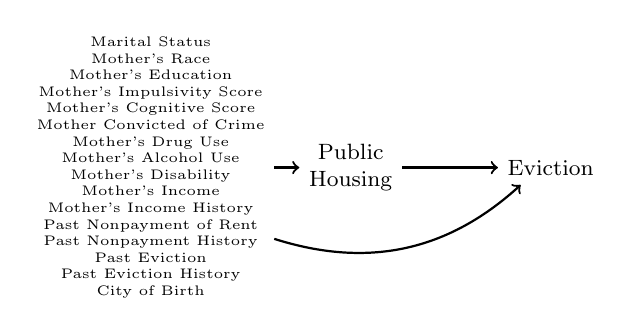
\begin{tikzpicture}[x = 1in, y = .5in]
\node[align = center, font = \tiny] (lag) at (-1,0) {Marital Status\\Mother's Race\\Mother's Education\\Mother's Impulsivity Score\\Mother's Cognitive Score\\Mother Convicted of Crime\\Mother's Drug Use\\Mother's Alcohol Use\\Mother's Disability\\Mother's Income\\Mother's Income History\\Past Nonpayment of Rent\\Past Nonpayment History\\Past Eviction\\Past Eviction History\\City of Birth};
\node[align = center, font = \footnotesize] (a) at (0,0) {Public\\Housing};
\node[align = center, font = \footnotesize] (y) at (1,0) {Eviction};
\draw[->, thick] (lag) -- (a);
\draw[->, thick] (a) -- (y);
\draw[->, thick] (lag) to[bend right] (y);
\end{tikzpicture} \vskip .1in \pause
Let's see how many strata have both
\begin{itemize}
\item Cases in public housing and
\item Cases with no assistance
\end{itemize}

\end{frame}

\begin{frame}{Conclusion: Positivity is deceptively hard to satisfy}
\pause

Positivity $\P(A = a\mid \vec{L} = \vec\ell) > 0$ may seem straightforward.\\ \pause
It quickly becomes difficult
\pause
\begin{itemize}[<+->]
\item Confounding may seem to require many covariates
\item But the more confounders, the harder positivity becomes\footnote{D'Amour, A., Ding, P., Feller, A., Lei, L., \& Sekhon, J. (2021). \href{https://doi.org/10.1016/j.jeconom.2019.10.014}{Overlap in observational studies with high-dimensional covariates}. Journal of Econometrics, 221(2), 644-654.}
\begin{itemize}
\item Tons of strata
\item Hard to populate all treatments in all of them
\end{itemize}
\item You end up leaning on a model to extrapolate (next class)
\end{itemize}
\end{frame}

\goalsframe

\begin{frame}{Let me know what you are thinking}

\begin{huge} \bref{https://tinyurl.com/CausalQuestions}{tinyurl.com/CausalQuestions} \end{huge}
\vskip .7in

Office hours TTh 11am-12pm and at \bref{https://calendly.com/ianlundberg/office-hours}{calendly.com/ianlundberg/office-hours}\\Come say hi!

\end{frame}

\end{document}

